% CNLSE
\documentclass[8pt,aspectratio=15,mathserif]{beamer} 
\setbeamertemplate{bibliography item}{\insertbiblabel}
% 设置段落间距
\setlength{\parskip}{0.3em}

\bibliographystyle{plain}
\usetheme{Dresden} %主题
\usepackage{setspace}
\usepackage{graphicx}
\usepackage{subfigure}
\usepackage{times}
\usepackage{amsmath}
\usepackage{url}
\usepackage{hyperref}
\usepackage{biblatex}
\addbibresource{mybib.bib}

% 超链接设置
\hypersetup{colorlinks = true, linkcolor = blue, anchorcolor = blue, citecolor = red}


% 设置行间距
%\renewcommand{\baselinestretch}{1.0}

\newtheorem{remark}{Remark}[section]


\mode<presentation>
{
 % 设置背景
 \setbeamertemplate{background canvas}[vertical shading][bottom=red!10,top=blue!10]
 
 % 设置block的特征
 \setbeamertemplate{blocks}[rounded][shadow=true]
 
 % 设置主题
 \usetheme{Warsaw}
 
 % 设置footline显示页码,但是由于warsaw本身已经定义了一个footline,所以这个定义就会覆盖warsaw的定义。另一方面说明,slides的每一部分都是可以自己定制的。
 % \setbeamertemplate{footline}[frame number]
 
% 添加页码代码,谷歌找到的。
\expandafter\def\expandafter\insertshorttitle\expandafter{%
    \insertshorttitle\hfill%
    \insertframenumber\,/\,\inserttotalframenumber}
 
 
 % 设置覆盖的效果,透明
 \setbeamercovered{transparent}
 
 \usefonttheme[onlysmall]{structurebold}
 
 % 设置数学公式的字体
 \usefonttheme[onlymath]{serif}
}
\title[Work Summary]{Solving PDE with deep learning}
\author[Xinyu Xiao]{Xinyu Xiao} % 显示作者
\institute[PKU]{Peking University} % 设置学院机构
\date{\today}  % 显示日期
    %\logo{\includegraphics[width=1.8cm,height=1.8cm]{1.png}}

\begin{document}

\begin{frame}
    \titlepage
\end{frame}


%%%%%%%%%%%%%%%%%%%%%%%%%%%%%%%%%%%%%%%%%
\frame {
    \frametitle{Table of Content}
    \tableofcontents
}

\section{A framework based deep learning}
\begin{frame}
\frametitle{DGM method \cite{DGM}}
Consider a PDE:
$$
\left\{\begin{array}{ll}
\left(\partial_{t}+\mathcal{L}\right) u(t, \boldsymbol{x})=0, & (t, \boldsymbol{x}) \in[0, T] \times \Omega \\
u(0, \boldsymbol{x})=u_{0}(\boldsymbol{x}), & \boldsymbol{x} \in \Omega \\
u(t, \boldsymbol{x})=g(t, \boldsymbol{x}), & (t, \boldsymbol{x}) \in[0, T] \times \partial \Omega
\end{array}\right.
$$
\begin{block}{Neural network approximation}
$$
u(x,t) \approx \hat{u}(x,t;\theta)
$$
\end{block}
\begin{block}{DGM loss}
\begin{align*}
J(\theta) &= loss_1 + loss_2 + loss_3 \\
loss_1 &= \left\|\frac{\partial \hat{u}}{\partial t}(t, x ; \theta) + \mathcal{L} \hat{u}(t, x ; \theta)\right\|_{[0, T] \times \Omega, \nu_{1}}^{2} \\
loss_2 &= \|\hat{u}(t, x ; \theta)-g(t, x)\|_{[0, T] \times \partial \Omega, \nu_{2}}^{2}\\
loss_3 &= \left\|\hat{u}(0, x ; \theta)-u_{0}(x)\right\|_{\Omega, \nu_{3}}^{2}
\end{align*}
\end{block}
\end{frame}

\begin{frame}
\frametitle{Why DGM method?}
In general, a Neural Network has form:
$$
\hat{u}(x,\theta) = \sum_{i=1}^{m} a_i \varphi(x;\theta_i)
$$
If we minimize 
$$
J(\theta) = <L\hat{u}-f,L\hat{u}-f>
$$
Then we can get:
\begin{align*}
\frac{\partial J}{\partial a_i} = <L\hat{u}-f,\varphi_i> = 0, \ i=1,2,\ldots,m
\end{align*}
which is exactly the Galerkin Method. So at this point of view, we can call this method as \textcolor{blue}{problem-driven spectral method}.
\end{frame}
\begin{frame}
\frametitle{Deep Ritz\cite{DeepRitz}}
Consider the Poisson equation:
\begin{align*}
-\Delta u&=f, x \in \Omega \\{}
u &=g,x \in \partial \Omega
\end{align*}
We can solve the optimization problem to get solution
\begin{block}{Ritz loss}
$$
J(u)=\int_{\Omega}\left(\frac{1}{2}\left|\nabla_{x} u(x)\right|^{2}-f(x) u(x)\right) d x+\beta \int_{\partial \Omega} (u(x)-g(x))^{2} d s
$$
\end{block}
\begin{block}{optimization}
$$
\hat{\theta} = \mathop{argmin} L(u(\cdot,\theta))
$$
\end{block}
\end{frame}

\begin{frame}
\frametitle{SGD}

\begin{block}{SGD}
When we can not consider the full batch gradient descent, we can use a batch gradient descent:
\begin{align*}
L(\theta) &= \int_{\Omega} h(x;\theta) dx \approx \frac{1}{N}\sum_{i=1}^{N}h(x_i,\theta)\\
\frac{\partial L}{\partial \theta} &= \int_{\Omega} \frac{\partial }{\partial \theta} h(x;\theta)dx \approx \frac{1}{N}\sum_{i=1}^{N} \frac{\partial }{\partial \theta}h(x_i,\theta)
\end{align*}
where $x_i$ are uniformly sampled on $\Omega$.
\end{block}

\begin{block}{PINN loss\cite{PINN}}
$$
R(x,t) = u_t + Lu
$$
$$
loss = MSE_u + MSE_f
$$
$$
M S E_{u}=\frac{1}{N_{u}} \sum_{i=1}^{N_{u}}\left|u\left(t_{u}^{i}, x_{u}^{i}\right)-u^{i}\right|^{2}, \quad M S E_{R}=\frac{1}{N_{f}} \sum_{i=1}^{N_{f}}\left|R\left(t_{f}^{i}, x_{f}^{i}\right)\right|^{2}
$$
\end{block}

\end{frame}


\begin{frame}
\frametitle{calculate differential operator}
In pytorch, we can calculate the differential operator in a direct manner.
\begin{figure}
\centering
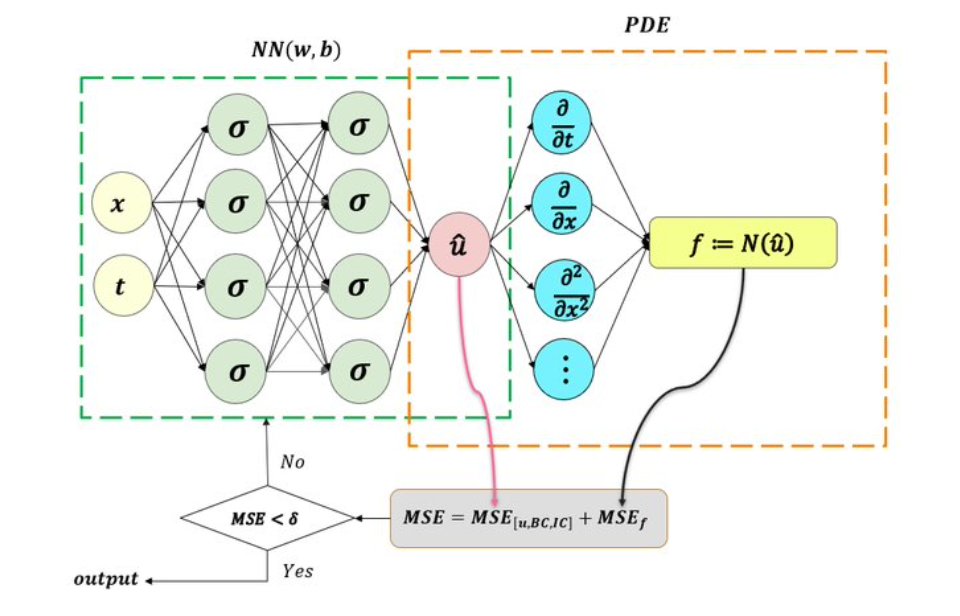
\includegraphics[width=0.6\linewidth]{img/PINN.png}
\caption{PINN\cite{PINN}}
\end{figure}
\end{frame}

\begin{frame}
\frametitle{calculate differential operator}
We can also calculate operator in a finite difference approximation.For example:
\begin{block}{Finite diffrence}\small
\begin{itemize}
\item time direction:Runge-kutta\cite{PINN}
$$
\begin{array}{l}
u^{n+c_{i}}=u^{n}-\Delta t \sum_{j=1}^{q} a_{i j} \mathcal{N}\left[u^{n+c_{j}}\right], \quad i=1, \ldots, q \\
u^{n+1}=u^{n}-\Delta t \sum_{j=1}^{q} b_{j} \mathcal{N}\left[u^{n+c_{j}}\right]
\end{array}
$$
\item space direction:\cite{DGM}
$$
\sum_{i, j=1}^{d} \rho_{i, j} \sigma_{i}(x) \sigma_{j}(x) \frac{\partial^{2} f}{\partial x_{i} x_{j}}(t, x ; \theta)=\lim _{\Delta \rightarrow 0} \mathbb{E}\left[\sum_{i=1}^{d} \frac{\frac{\partial f}{\partial x_{i}}\left(t, x+\sigma(x) W_{\Delta} ; \theta\right)-\frac{\partial f}{\partial x_{i}}(t, x ; \theta)}{\Delta} \sigma_{i}(x) W_{\Delta}^{i}\right]
$$
\end{itemize}
\end{block}
\end{frame}

\begin{frame}
\frametitle{sampling trick:Latin Hypercube Sampling strategy}
In Latin Hypercube sampling is similar to having N rooks on a chess board without threatening each other.[Wiki]
\begin{figure}
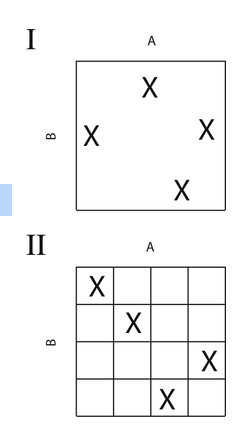
\includegraphics[width=0.22\linewidth]{img/chess.png}
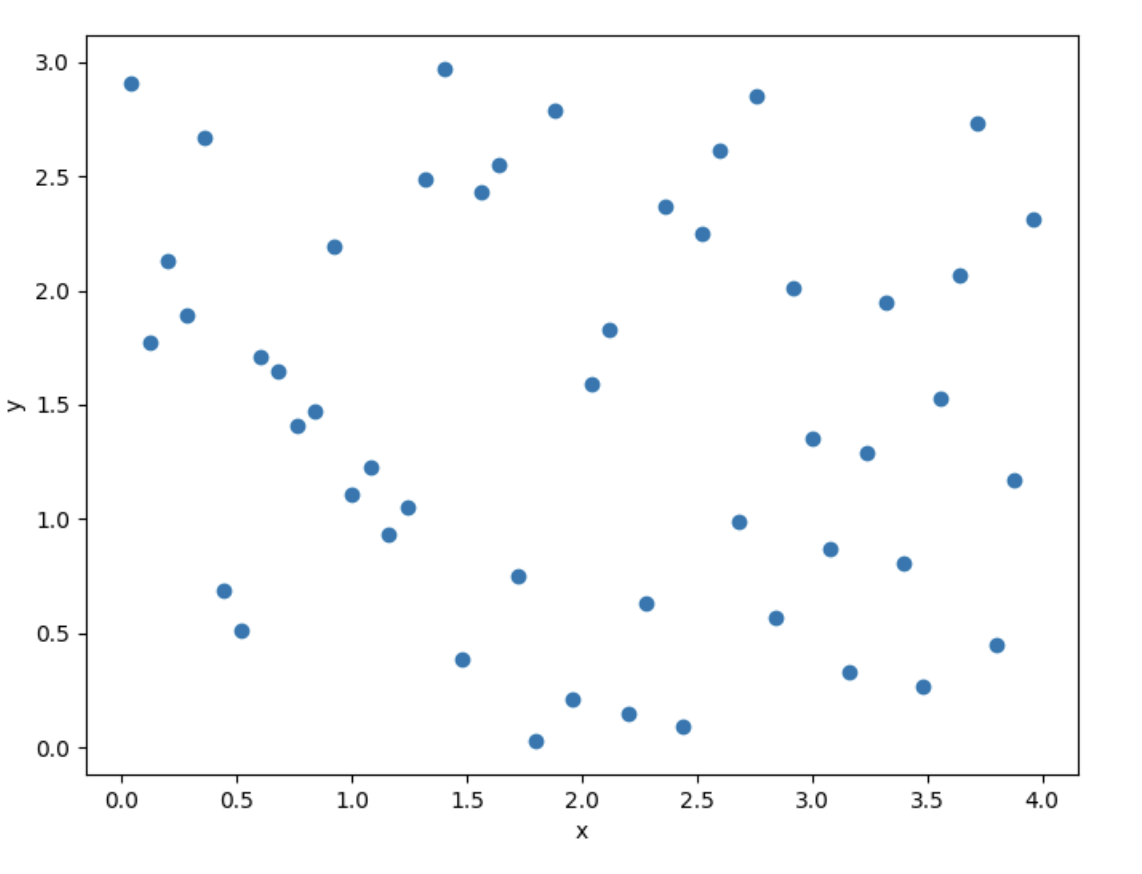
\includegraphics[width=0.5\linewidth]{img/sampling.png}
\end{figure}
We can use more sampling trick here such as \textcolor{blue}{importance sampling} and \textcolor{blue}{MCMC}.
\end{frame}

\frame {
    \frametitle{Table of Content}
    \tableofcontents
}
\section{Numerical result}
\subsection{A Nonlinear case}
\begin{frame}
\frametitle{Burgers equation}
\begin{figure}
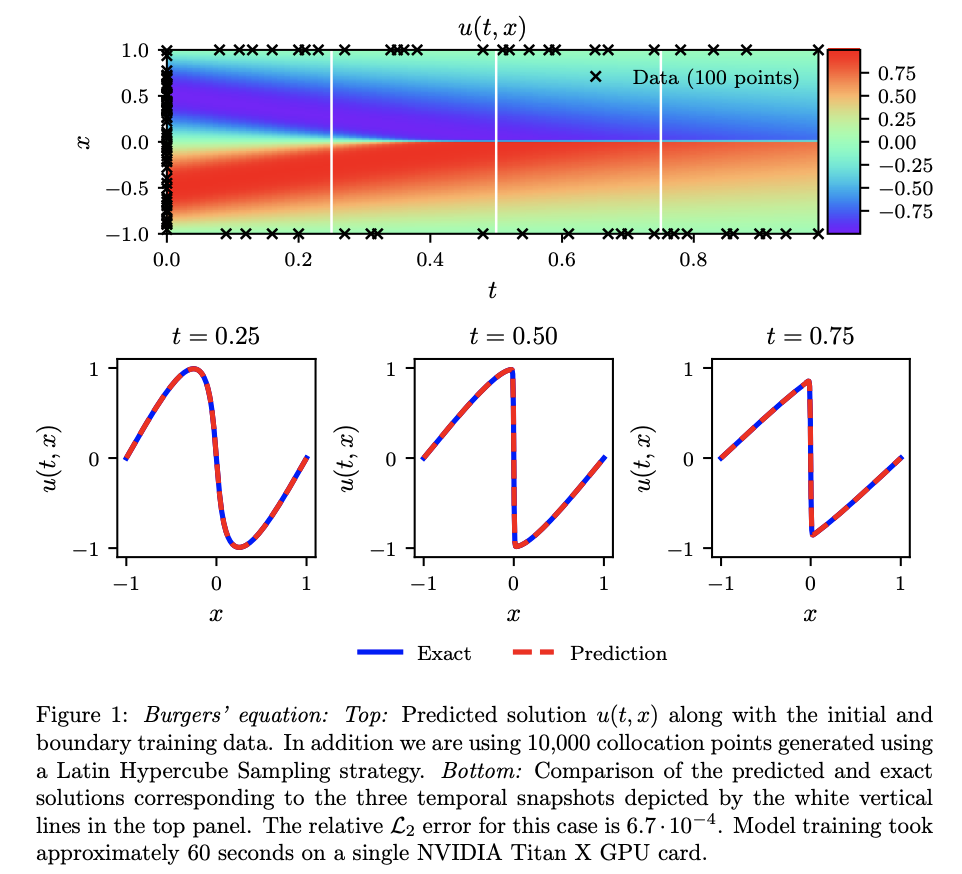
\includegraphics[width=0.65\linewidth]{img/Burgers.png}
\caption{result from \cite{PINN}}
\end{figure}
\end{frame}

\begin{frame}
\frametitle{Burgers equation:systematic studies}
\begin{figure}
\centering
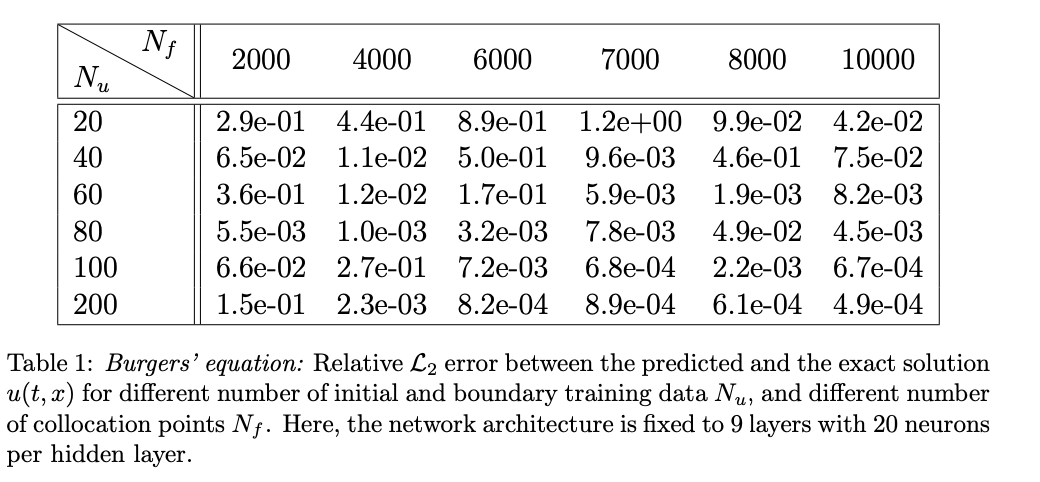
\includegraphics[width=0.8\linewidth]{img/Table1.png}
\caption{result from \cite{PINN}}
\end{figure}
\end{frame}

\begin{frame}
\frametitle{Burgers equation:systematic studies}
\begin{figure}
\centering
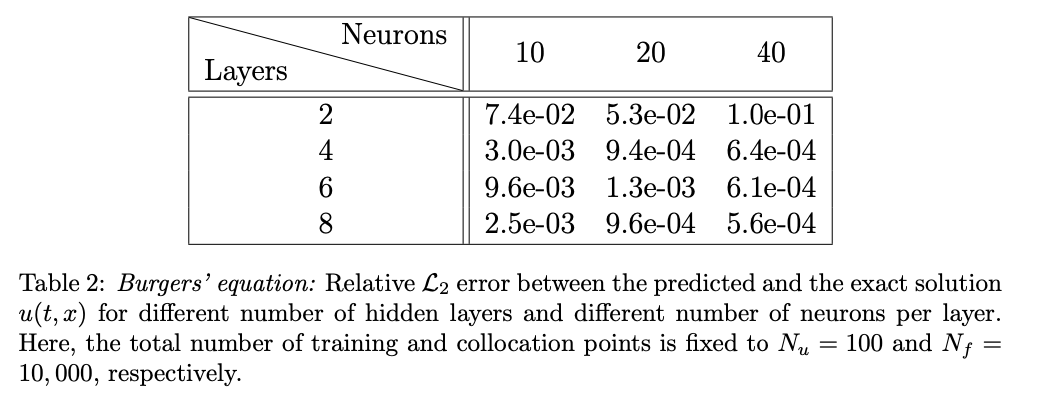
\includegraphics[width=0.8\linewidth]{img/Table2.png}
\caption{result from \cite{PINN}}
\end{figure}
\end{frame}

\subsection{High dimensional case}
\begin{frame}
\frametitle{A High dimensional case}
\begin{block}{Helmoholz equation}
$\Omega=[0,1]^d$.
$$
-\Delta u+\pi^{2} u=f(x)
$$
\end{block}
\begin{definition}[relative L2 error]
$$
\text { error }=\left(\int_{\Omega}\left(u^{*}\left(x ; \theta^{*}\right)-u(x)\right)^{2} \mathrm{~d} x\right)^{\frac{1}{2}} \cdot\left(\int_{\Omega}(u(x))^{2} \mathrm{~d} x\right)^{-\frac{1}{2}}
$$
\end{definition}
The paper \cite{Compare} compared the performance of DGM and Deepritz.
\begin{figure}
\centering
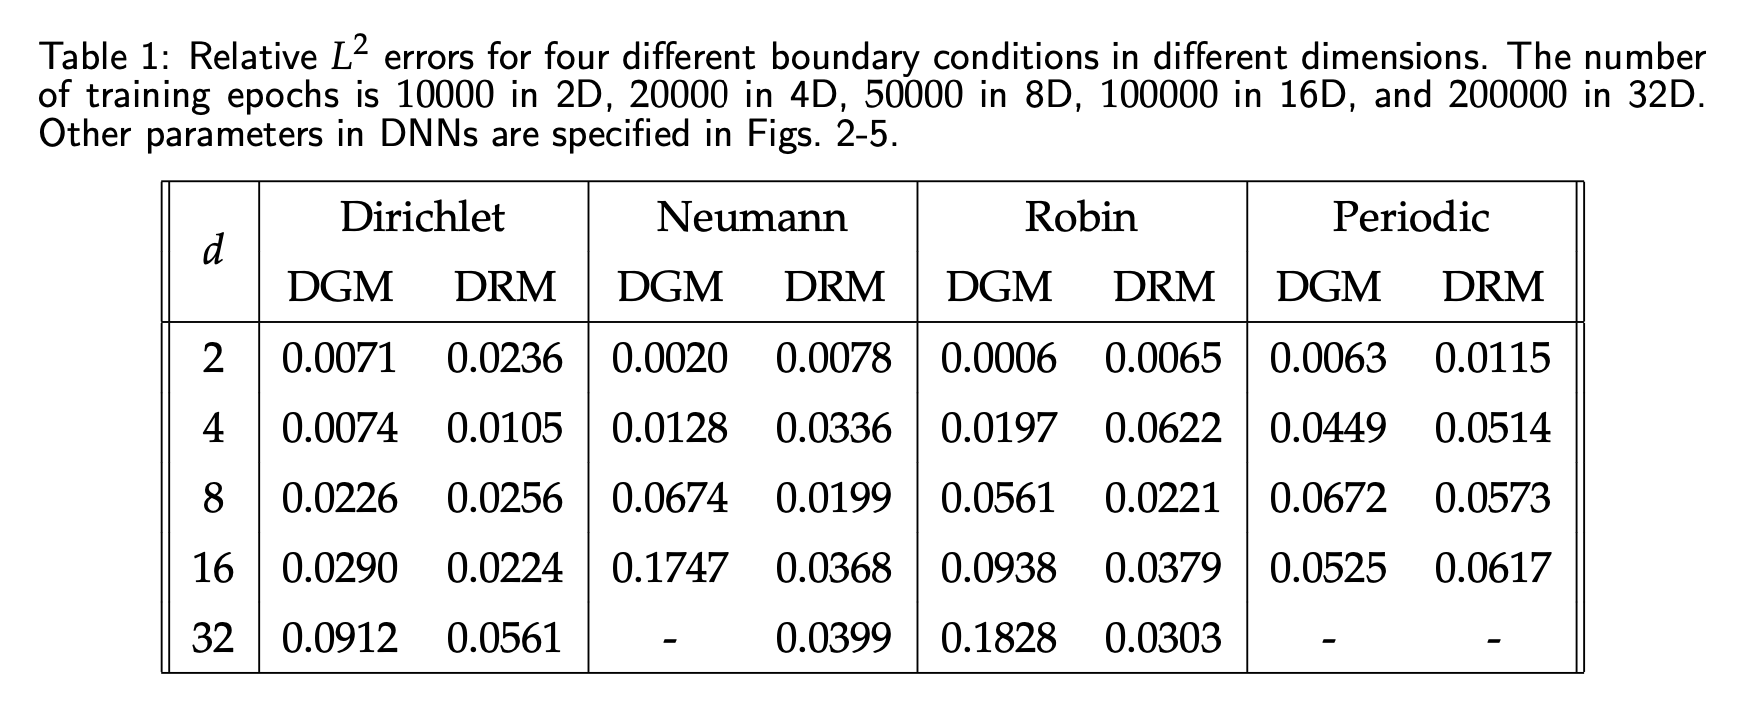
\includegraphics[width=0.7\linewidth]{img/high_Poisson.png}
\end{figure}
\end{frame}


\begin{frame}
\frametitle{Disccusion}
Advantage:
\begin{itemize}
\item meshfree: a path to high-dimensional PDE.
\item handle complex region.
\end{itemize}
Disadvantage:
\begin{itemize}
\item No convergence theorem.
\item Low precision compared with classical method(FEM,spectral method).
\end{itemize}
\end{frame}

\frame {
    \frametitle{Table of Content}
    \tableofcontents
}
\section{Some improvement}
\subsection{Penalty free method}
\begin{frame}
\frametitle{PFNN:Penalty free NN}
While we do not want to introduce penalty terms for boundary conditions, we can use a \textcolor{blue}{penalty free} method\cite{Penalty_free}.
$$
w_{\boldsymbol{\theta}}(\boldsymbol{x})=g_{\boldsymbol{\theta}_{\mathbf{1}}}(\boldsymbol{x})+\ell(\boldsymbol{x}) f_{\boldsymbol{\theta}_{\mathbf{2}}}(\boldsymbol{x})
$$
where $l(x)$ is a index function(perhaps a distance function to boundary).
$$
\left\{\begin{array}{ll}
\ell(\boldsymbol{x})=0, & \boldsymbol{x} \in \Gamma_{D} \\
\ell(\boldsymbol{x})>0, & \text { otherwise. }
\end{array}\right.
$$
Two neural networks, one for boundary conditions, another for internal points. In this way, we can solve two optimization problems without constrain.
\end{frame}

\begin{frame}
\frametitle{100D cube poission-like equtions}
$$
\left\{\begin{aligned}
-\nabla \cdot\left(|\nabla u|^{p-2} \nabla u\right)+u+c &=0, \quad \text { in } \Omega \\
u &=\varphi, \quad \text { on } \Gamma_{D} \\
\left(|\nabla u|^{p-2} \nabla u\right) \cdot \boldsymbol{n}+\alpha u &=\psi, \quad \text { on } \Gamma_{R}
\end{aligned}\right.
$$
\begin{figure}
\centering
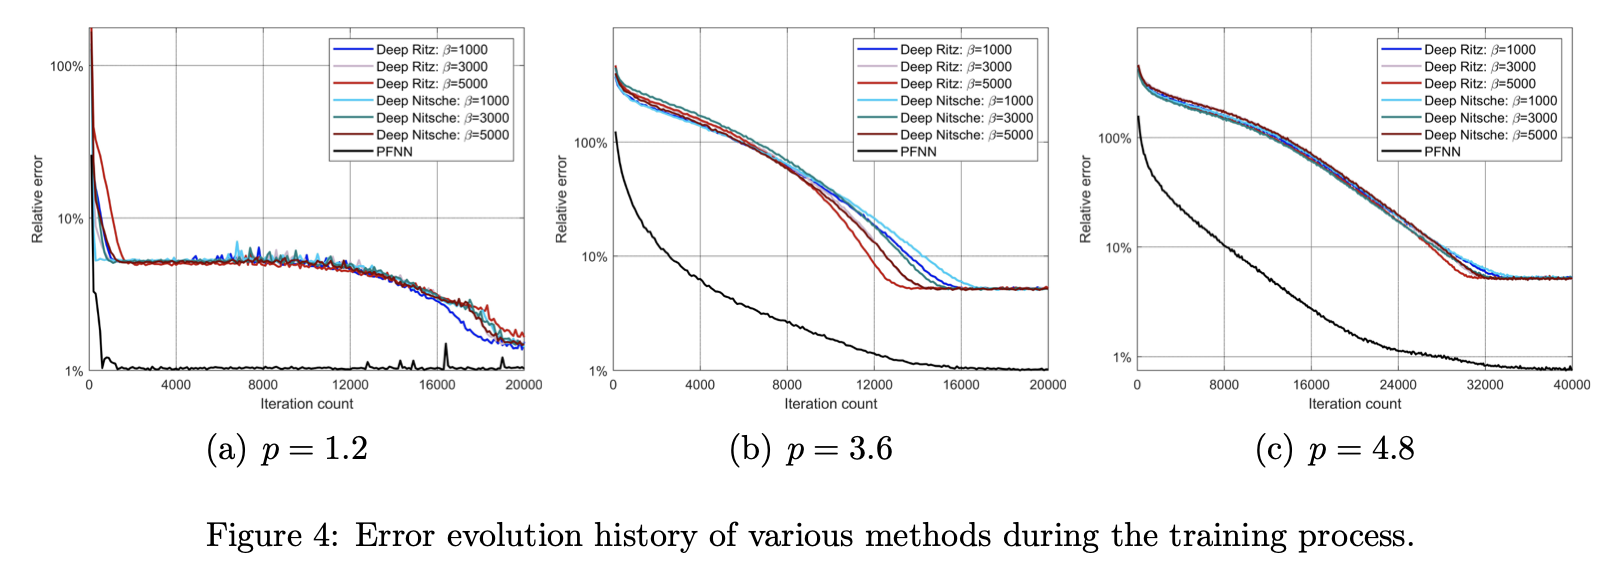
\includegraphics[width=1.0\linewidth]{img/PFNN.png}
\caption{region}
\end{figure}
\end{frame}

\begin{frame}
\frametitle{complex region}
\begin{figure}
\centering
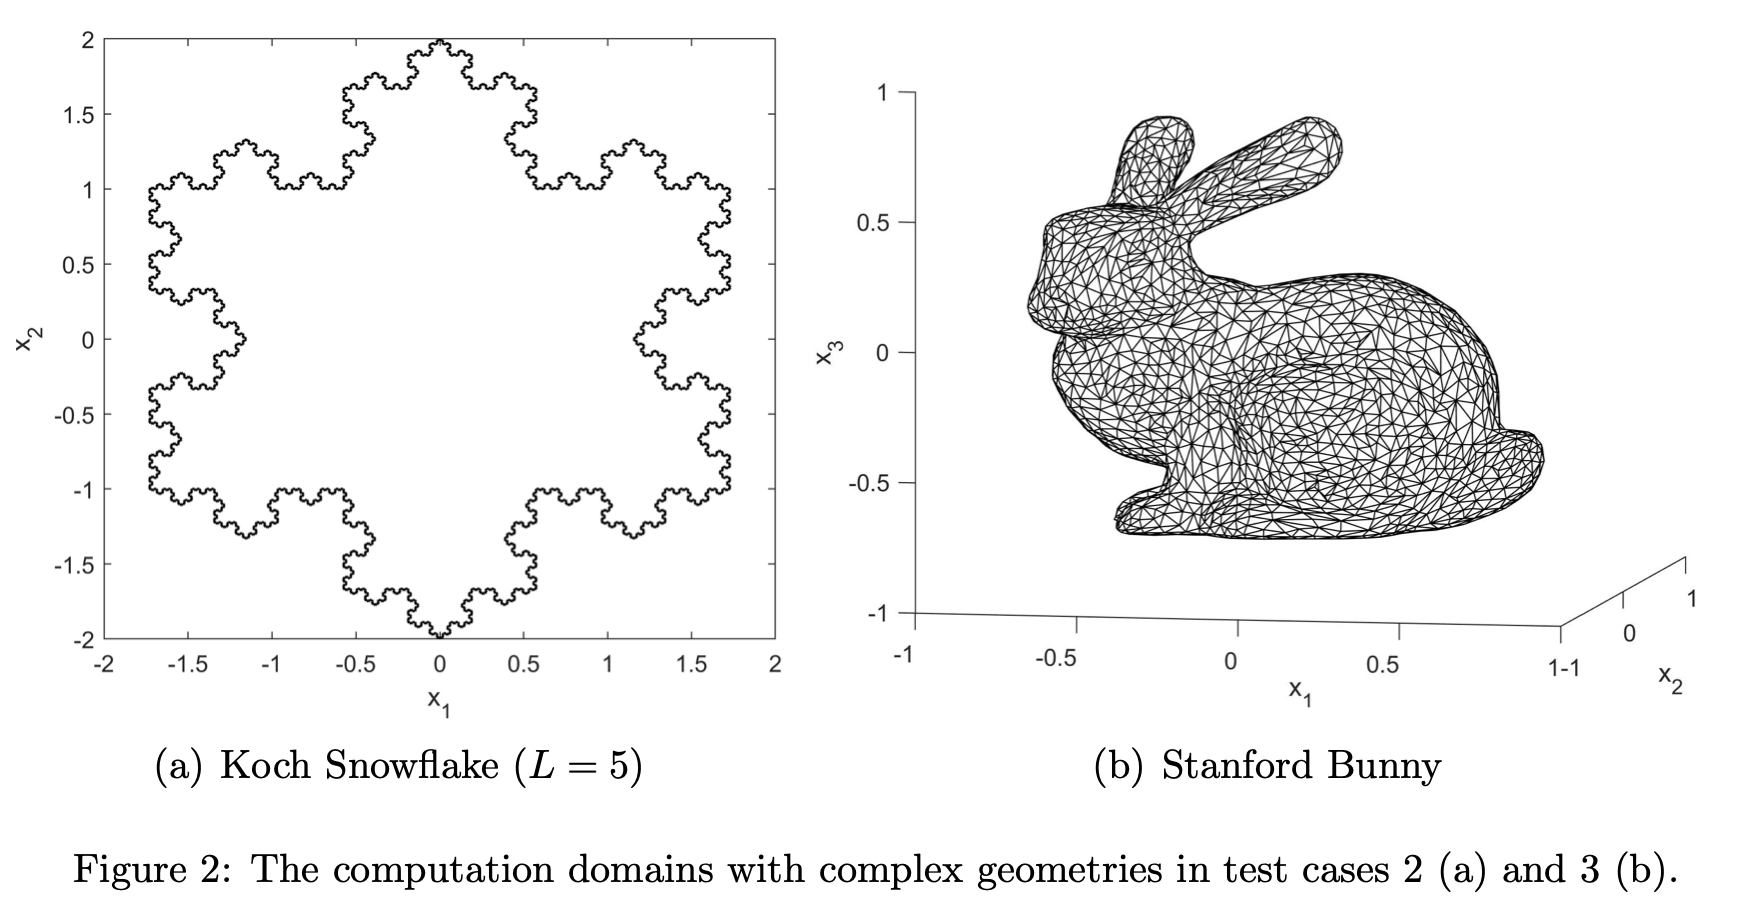
\includegraphics[width=0.8\linewidth]{img/complex_region.png}
\caption{region}
\end{figure}
\end{frame}

\subsection{Fourier feature embeddings}
\begin{frame}
\frametitle{Fourier feature embeddings}
\cite{FT_embedding} show that we can introduce a fourier embedding layer to solve multi-scale problem.
\begin{figure}
\centering
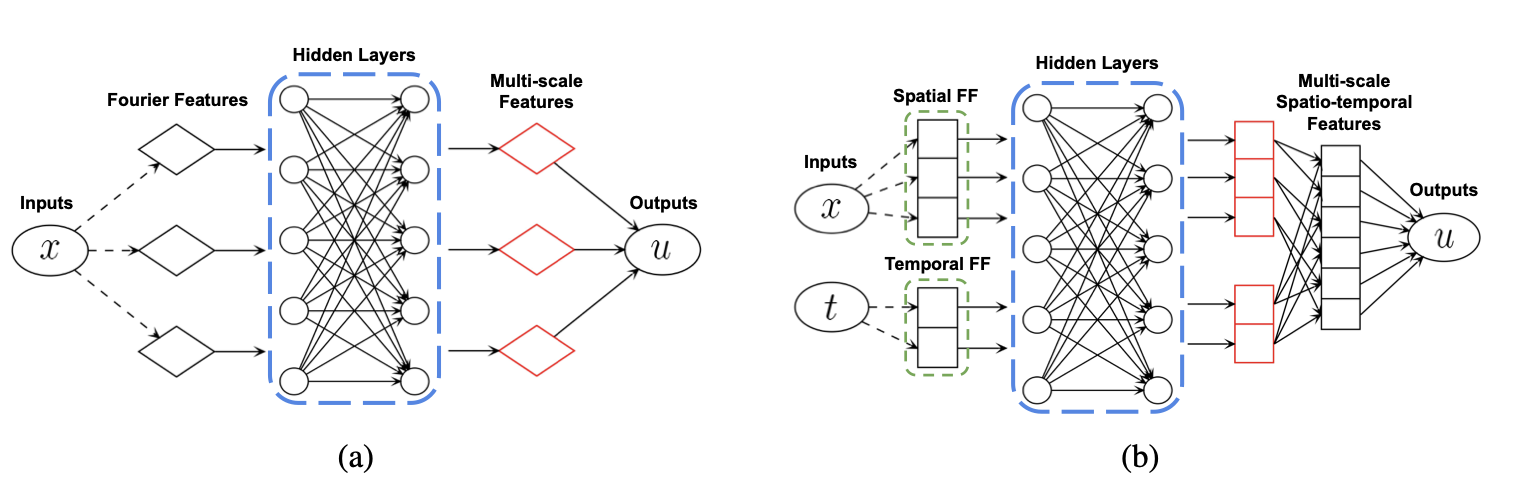
\includegraphics[width=0.8\linewidth]{img/Fourier_embedding.png}
\end{figure}
\begin{block}{Fourier embedding}
$$
\gamma^{(i)}(\boldsymbol{x})=\left[\begin{array}{l}
\cos \left(2 \pi \boldsymbol{B}^{(i)} \boldsymbol{x}\right) \\
\sin \left(2 \pi \boldsymbol{B}^{(i)} \boldsymbol{x}\right)
\end{array}\right]
$$
\end{block}
\end{frame}
\newpage
\printbibliography{unsrt}
\end{document}
